\documentclass[style=aggie]{powerdot}

\usepackage[utf8]{inputenc}

\pdsetup{}

\title{bioremediation and the cracked crystall ball}
\author{Stephan Richter}
\date{2013-04-30}

\begin{document}
\maketitle

\begin{slide}{Overview}
\tableofcontents[content=sections]
\end{slide}

\section{Motivation}
\begin{slide}{Situation}
\begin{itemize}
 \item many former industrial sites
 \item toxic pollutants sept into the soil for years/decades
 \includegraphics[width=0.8\textwidth]{waggon.ps}
 \item substances still there, resist degradation
 \item for some substances: degraders known
\end{itemize}
\end{slide}

\begin{slide}{Idea: Faciliation of BIOREMEDIATION using MULTIPLE BACTERIAL SPECIES}
\begin{itemize}
 \item potential degrading bacteria known\\ (at least for some contaminants)\newline
 \item how can we take advantage of those bacteria?\newline
 \item can't we use them for faciliation of contaminat removal?\newline
 \item what additions are needed?\newline
 \item what are the side products of pollutant mineralization?\newline
 \item what can we do about the side products?
\end{itemize}
\end{slide}

\begin{slide}{Idea: What are we aiming for?}
\begin{itemize}
 \item input: soil situation
 \begin{itemize}
  \item pH
  \item himudity
  \item oxygen level
  \item temperature
  \item salinity
  \item present bacteria
   \newline
 \end{itemize}

 \item desired \textbf{toolbox} output: \textbf{solution strategy}
 \begin{itemize}
  \item bacteria to introduce
  \item micronutrients to supply
 \end{itemize}

\end{itemize}
\end{slide}

\section{Toolbox development}

\begin{slide}{Main functionality}
\begin{itemize}
 \item identify potential degraders in online databases
 \item identify intermediates and dead end products
 \item identify degraders for intermediates/dead end products
 \item \textcolor{gray}{determine optimal set of bacteria\footnote{not implemented, yet}}
 \item \textcolor{gray}{design wet land experiments for verification\footnotemark[1]}
\end{itemize}
\indent $\Rightarrow$ multi-species bacterial networks
\end{slide}

\end{document}
